\documentclass[12pt,a4j]{jarticle}
\floatsep=10mm
\textfloatsep=10mm
\usepackage[dvips]{graphicx}
\usepackage{graphicx}
\usepackage{amscd}
\usepackage{multirow}
\usepackage{epsfig}
\usepackage{amsmath,amssymb,epsf}
\usepackage{comment}
\usepackage{graphicx,psfrag}
\usepackage{bm}
\def\vec#1{\mbox{\boldmath$#1$}}
\def\sgn#1{\mbox{sgn($#1$)}}
\def\c#1{^{#1}}
\def\argmin#1{\underset{#1}{\mbox{argmin}}}
\def\leqq{\le}
\def\geqq{\ge}
%%%$B%Z!<%8%l%$%"%&%H$N%W%j%"%s%V%k(B%%%%
\setlength{\unitlength}{1mm}
\setlength{\topmargin}{-1cm}
\setlength{\oddsidemargin}{-0.55cm}
\setlength{\evensidemargin}{-0.55cm}
\setlength{\textheight}{24cm}
\setlength{\textwidth}{17cm}
\renewcommand{\baselinestretch}{1.3}

%%%%%%%%%%%%%$B?^I=$N3d9g(B%%%%%%%%%%%%%%%
\setcounter{topnumber}{5}%    $B%Z!<%8>eIt$N?^I=$O(B 5 $B8D$^$G(B
\def\topfraction{1.00}%       $B%Z!<%8$N>e(B 1.00 $B$^$G?^I=$G@j$a$F2D(B
\setcounter{bottomnumber}{5}% $B%Z!<%82<It$N?^I=$O(B 5 $B8D$^$G(B
\def\bottomfraction{1.00}%    $B%Z!<%8$N2<(B 1.00 $B$^$G?^I=$G@j$a$F2D(B
\setcounter{totalnumber}{10}% $B%Z!<%8$"$?$j$N?^I=$O(B 10 $B8D$^$G(B
\def\textfraction{0.1}%      $B%Z!<%8$&$AK\J8$,@j$a$k3d9g$N2<8B(B
\def\floatpagefraction{0.6}%  $B?^I=$@$1$N%Z!<%8$O>/$J$/$H$b$3$l$@$1$r?^I=$,@j$a$k(B


%\documentclass[12pt,a4j,epsf,amstex,righttag]{jarticle}
%%%%%%%%%%%% $B0J2<$O(BLinux $B$N(B Latex2e $B$G%3%s%Q%$%k$9$k$H$-(B
% rcp hirata.tex izanagi:~/tex/sotu/sotu98/
%%%%%%%%%%%% (mule$B$G$N%-!<A`:n$O(B^ctj)

%%%%%%%%%%%%% $B0J2<$O(BUnix $B$N(B amslatex $B$G%3%s%Q%$%k$9$k$H$-(B
%\documentstyle[12pt,a4j,epsf,amstex,righttag]{jarticle}
%\def\myepsfile#1#2#3{\epsfile{file=#1,width=#2}}
%%%%%%%%%%%%% $B0J>e$O(BUnix $B$N(B amslatex $B$G%3%s%Q%$%k$9$k$H$-(B

% $B%0%i%U%#%C%/%9$N;HMQ(B
%\usepackage[dvips]{graphicx}
% -- AMS$B%Q%C%1!<%8!&(BAMSFonts
%\usepackage{amsmath,amssymb}
% $B?t<0MQ%U%)%s%H(B
%\\usepackage{mathptmx}
%\setlength{\topmargin}{.5cm}
%\setlength{\unitlength}{1mm}
\def\dint_#1^#2{\displaystyle{\int_{#1}^{#2}}}
\def\tint_#1^#2{\textstyle{\int_{#1}^{#2}}}
\def\dfrac#1#2{\displaystyle{\frac{#1}{#2}}}
\def\tfrac#1#2{\textstyle{\frac{#1}{#2}}}
\def\textem#1{\textit#1}
\def\vec#1{\mbox{\boldmath$#1$}}
\def\argmin#1{\underset{#1}{\mbox{argmin~}}}
\def\argmax#1{\underset{#1}{\mbox{argmax~}}}
\def\RealNumSet{\Bbb R}
%\def\exp#1{e^{#1}}
%\def\eqn#1{(\ref{#1})}
%\def\refeq#1{$B<0(B(\ref{#1})}
%\def\reffig#1{$B?^(B\ref{#1}}
%\def\reftab#1{$BI=(B\ref{#1}}
%\def\aratio{\theta_{\alpha}}
%\def\eratio{\theta_{H}}
%\def\reinitratio{\theta_{r}}
%\renewcommand{\floatpagefraction}{1}
%\renewcommand{\topfraction}{1}
%\renewcommand{\bottomfraction}{1}
%\renewcommand{\textfraction}{0}
%\renewcommand{\theequation}{\thesubsection.\arabic{equation}}
\def\bg{{\bf{bg}}}
\def\ob{{\bf{ob}}}
\def\ib{{\bf{ib}}}
\def\tst{{\bf{tst}}}
\def\bst{{\bf{bst}}}
\def\tr{{\bf{tr}}}
\def\bs{{\bf{bs}}}
\def\bb{{\bf{bb}}}
\def\mse{{\bf{MSE}}}
\def\mae{{\bf{MAE}}}
\def\mxae{{\bf{MxAE}}}

\begin{document}




\section{Kinect$B%;%s%5$HCO<'5$J}0L%;%s%5$*$h$SCO?^>pJs$rMQ$$$k%Q!<%F%#%/%k%U%#%k%?$K$h$k<+8J;Q@*?dDj(B}
 \subsection{$BCO?^>pJs$rMQ$$$k(BPF$B$K$h$k<+8J;Q@*?dDj(B}
  \subsubsection{$BCO?^>pJs$N:n@.(B}
  $BK\8&5f$GMQ$$$kCO?^>pJs$O%0!<%0%k%^%C%W$rMQ$$$F:n@.$9$k!%%0!<%0%k%^%C%W$h$j(B, $B<B:]$KAv9T$7$?F;O)(B
$B$NCf1{IU6a$NJ#?tE@$N0^EY(B, $B7PEY$r<hF@$7(B, $BKL$r(B$y$$B<4J}8~(B, $BEl$r(B$x$$B<4J}8~$H$7(B
$B$?@$3&:BI8$X$HJQ49$9$k(B. $B;~9o(B$k$$B$G$NKL0^!$(B
$BEl7P$r(B$N_{k}$$B!$(B$E_{k}$$B$H$9$k$H!$El7P$NJQ49$O(B
\begin{equation}
 x_{k}
  =(E_{k}-E_{0})
  \frac{\beta}{360}\
  cos\left(\frac{\pi N_{0}}{180}\right)
\end{equation}
$B$H$J$k!%$3$3$G(B$\beta$$B$O@VF;D9$G(B$40075.017$[km]$B$G$"$k!%F1;~$KKL0^$O(B
\begin{equation}
 y_{k}=(N_{k}-N_{0})\frac{\pi\gamma}{360}
\end{equation}
$B$H$J$k!%$3$3$G(B$\gamma$$B$OKL6K$HFn6K$r7k$s$@D>7B$G(B$12756.274$[km]$B$G$"$k!%(B


$B<hF@$7$?E@(B$\vec{m}_{i}=({x_i},{y_i})(i=1,2,3,4,5)$$B$r7k$S(B,
$BCO?^>pJs(B${\it{R}}=\{\vec{x} \mid
\vec{x}=\alpha(\vec{m}_{j+1}-\vec{m}_{j})+\vec{m}_{j}\}(0<\alpha\leq 1,
j=1,2,3,4 , \vec{m}_{5}=\vec{m}_{1})$
$B$H$7$F;HMQ$9$k!%:n@.$7$?7PO)>pJs$r%0!<%0%k%^%C%W$KI=<($7$??^$r?^(B\ref{$BCO?^>pJs(B}$B$K<($9!%(B

\begin{figure}[h]
 \begin{center}
  \begin{tabular}{cc}
   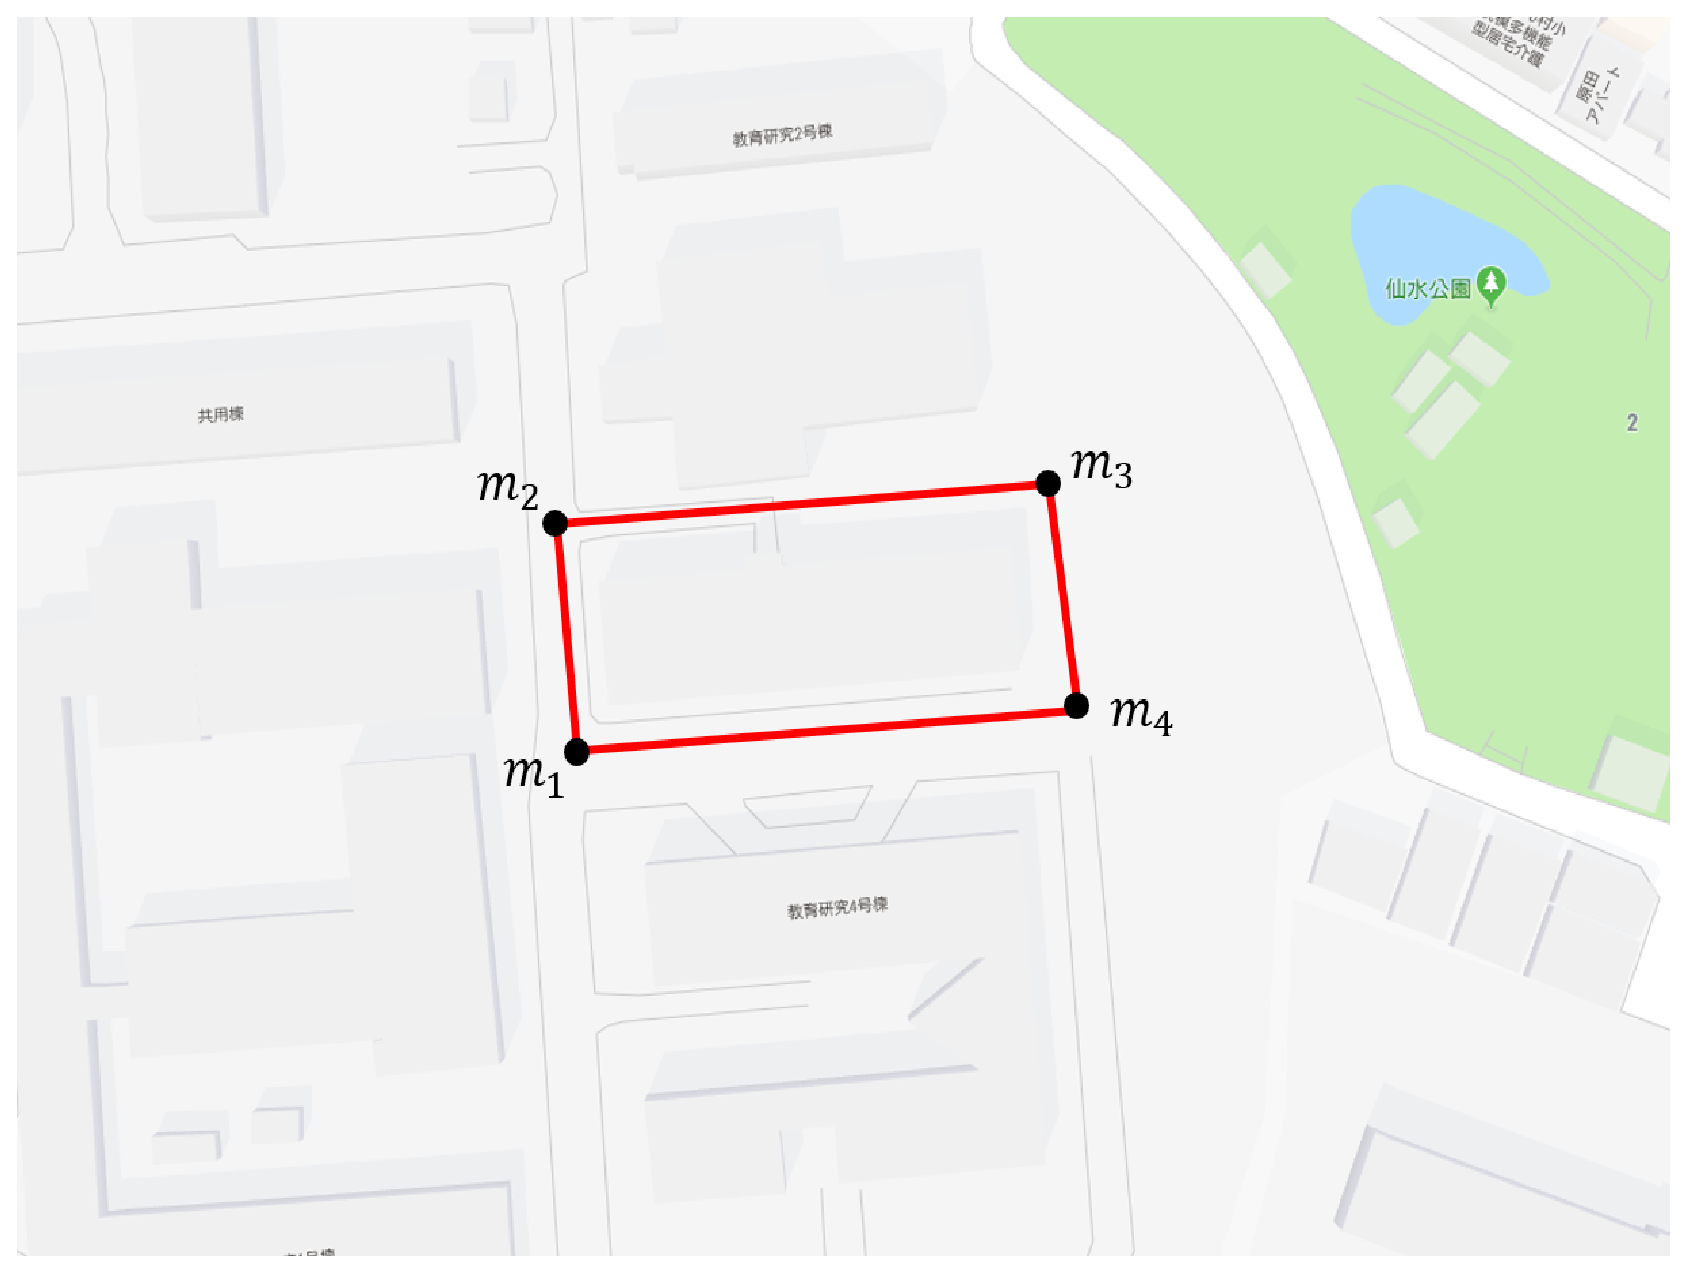
\includegraphics [height=5.0cm,width=8.0cm] {./fig/gpst.eps}
  \end{tabular}
 \end{center}
 \caption{$BCO?^>pJs(B}\label{$BCO?^>pJs(B}
\end{figure}
\clearpage
\newpage
  \subsubsection{PF$B$K$h$k<+8J;Q@*?dDj%"%k%4%j%:%`(B}
  $B%Q!<%F%#%/%k%U%#%k%?(B(PF)$B$H$O3NN(L)EYJ,I[$rB??t$N%5%s%W%k$K$h$C$F6a;w$9$k<jK!$N0l$D$G$"$k!%>uBV6u4VCf$N%Q!<%F%#%/%k$H8F$P$l$kB??t$NN3;R$K$h$j!$%m%\%C%H$N;Q@*$K4X$9$k2>@b$rJ#(B
$B?tN)$F$k$3$H$K$h$jJ,I[$r6a;w$7!$$=$l$rDI@W!$;~4V99?7$9$k%"%k%4%j%:%`$G$"(B
$B$k!%K\8&5f$G<BAu$9$k(BPF$B$N%"%k%4%j%:%`$r0J2<$K4J7i$K<($9!%>0!$K\8&5f$K9g$o(B
$B$;$F2f!9$N8&5f(B
$B<<$G=>Mh$N<+8J;Q@*?dDj$KMQ$$$i$l$F$$$?$b$N$r2~NI$7$F$*$j!$@h9T8&5fO@J8$G$b(B
$B>R2p$5$l$F$$$k$b$N$r0lIt;29M$K$7$F$$$k!%(B[1]\\
 $B$^$:!$;~9o(B$k-1$$B$G$N%m%\%C%H$N;Q@*$r(B
 $\vec{x}_{k-1}=(x_{k-1},y_{k-1},\theta_{k-1})^T$$B$H$7!$$=$N;~9o$N;Q@*$K(B
 $B$D$$$F$N3F%Q!<%F%#%/%k$NJ,I[$r(B$r(\vec{x}_{k-1})$$B$H$9$k!%$3$N$H$-!$%Q!<%F%#%/%k72(B
$\bigl< \vec{X}_{k-1}^{[m]} \bigr>_{m=1}^{M}$$B$K$h$k6a;w$O(B
$\bigl< \vec{X}_{k-1}^{[m]} \bigr>_{m=1}^{M}
=\bigl<\vec{x}_{k-1}^{[m]},w_{k-1}^{[m]} \bigr>_{m=1}^{M}$
$B$N$h$&$KM?$($i$l$F$$$k$b$N$H$9$k!%$3$3$G!$(B$M$$B$O%Q!<%F%#%/%k?t$G$"$j!$3F!9(B
$B$N;Q@*(B$\vec{x}_{k-1}^{[m]}$$B$H$=$N=E$_(B($BL`EY(B)$w_{k-1}^{[m]}$$B$r$b$DJ#?t$N%Q!<(B
$B%F%#%/%k$K$h$j!$%Q!<%F%#%/%k72$,9=@.$5$l$k!%$3$3$G>eE:;z(B$[m](m=1,2,\cdots,M)$
$B$O%Q!<%F%#%/%k$N%$%s%G%C%/%9$rI=$7$F$*$j!$3F=E$_(B$w_{k-1}^{[m]}$$B$O(B
$0 \leq w_{k-1}^{[m]} \leq 1$$B!$(B$\sum_{m=1}^{[M]} w_{k-1}^{[m]}=1$
$B$rK~$?$9$b$N$H$9$k!%(B\par
PF$B$O0J2<$N(B$3$$B%9%F%C%W$N=hM}$r9T$&!%$?$@$7!$;~9o(B$0$$B$K$*$1$k=i4|>uBV$K$D$$$F$O(B
$B$9$Y$F$N%Q!<%F%#%/%k$KBP$7!$(B
$\bigl< \vec{X}_{0}^{[m]} \bigr>_{m=1}^{M}
=\bigl< \vec{x}_{0}^{[m]},w_{0}^{[m]} \bigr>_{m=1}^{M}
=\bigl< (0,0,0)^T,\frac{1}{M} \bigr>_{m=1}^{M}$
$B$HM?$($F$*$/$b$N$H$9$k!%(B
\begin{enumerate}
 \item[Step 1:]{\bf $B;Q@*?dDj(B}\par
$B;~9o(B$k-1$$B$K$*$1$k;Q@*(B$\vec{x}_{k-1}^{[m]}$$B$H%m%\%C%H$N@)8fF~NO(B
$\vec{u}_{k-1}$$B$,M?$($i$l$?2<$G!$<!;~9o(B$k$$B$K$*$1$k;Q@*(B$\vec{x}_k$
$B$K4X$9$kDs0FJ,I[(B$\tilde{q}(\vec{x}_k)$$B$K=E$_(B$w$$B$rIU2C$7!$%Q!<%F%#%/%k72(B
$\bigl< \tilde{\vec{X}}_{k}^{[m]} \bigr>_{m=1}^M
=\bigl< (\tilde{\vec{x}}_{k}^{[m]},\tilde{w}_{k}^{[m]}) \bigr>_{m=1}^{M}$
$B$r@8@.$9$k!%$3$N=hM}$OK\O@J8$NIUO?(BA$B$K=R$Y$F$$$k%m%\%C%H$NB.EYF0:n%b%G%k$rMQ$$$F!$<!;~9o$KCV$1$k%m%\%C%H$N;Q@*$N2>@b$rJ#?t%5%s%W%j%s%0$9$k$b$N$G$"$k!%$D$^$j!$3F%Q!<%F%#%/%k$4$H$K%m%\%C(B
	       $B%H$N@)8fF~NO$K0[$J$k%N%$%:$r2C$(?7$?$J@)8fF~NO(B
$\hat{\vec{u}}_{k-1}^{[m]}=(\hat{v}_{k-1}^{[m]},\hat{\omega}_{k-1}^{[m]})^T
=(v_{k-1}+\varepsilon^{[m]},\omega_{k-1}+\varepsilon^{[m]})^T$
$B$r@8@.$9$k$3$H$G!$(B$\hat{\omega}_{k-1}^{[m]} \neq 0$$B$N$H$-$N(B
$B<!;~9o$K$*$1$k;Q@*$N2>@b(B$\tilde{\vec{x}}_{k}^{[m]}$$B$,<!<0$N$h$&$K5a$a$i(B
$B$l$k!%(B
\begin{equation}
 \tilde{\vec{x}}_{k}^{[m]}=\vec{x}_{k-1}^{[m]}+\left(
					      \begin{array}{c}
					       -\frac{\hat{v}_{k-1}^{[m]}}{\hat{\omega}_{k-1}^{[m]}}
						\sin{\theta_{k-1}^{[m]}}
						+\frac{\hat{v}_{k-1}^{[m]}}{\hat{\omega}_{k-1}^{[m]}}
						\sin{(\theta_{k-1}^{[m]}+\hat{\omega}_{k-1}^{[m]}\Delta
						t_{k-1})}\\
					       \frac{\hat{v}_{k-1}^{[m]}}{\hat{\omega}_{k-1}^{[m]}}
						\cos{\theta_{k-1}^{[m]}}
						-\frac{\hat{v}_{k-1}^{[m]}}{\hat{\omega}_{k-1}^{[m]}}
						\cos{(\theta_{k-1}^{[m]}+\hat{\omega}_{k-1}^{[m]}\Delta
						t_{k-1})}\\
					       \hat{\omega}_{k-1}^{[m]}\Delta
						t_{k-1}\\
					      \end{array}
					     \right)
\end{equation}\\
 \item[Step 2:]{\bf $B=E$_(B($BL`EY(B)$B$N7W;;(B}\par
$BJ}0L%;%s%5$H(BKinect$B%;%s%5$N7WB,>pJs$rMQ$$$F!$B.EYF0:n%b%G%k$K$h$C$F5a$a$i$l$?(B
$B8=:_$N;Q@*?dDjCM(B
$\tilde{\vec{x}}_{k}^{[m]}$
$B$H$N%^%C%A%s%0$K$h$jJ,I[$N=E$_(B($BL`EY(B)$B$r7W;;$9$k!%(B
$BJ}0L%;%s%5$N7WB,CM$r(B$\theta_k$$B$H$9$k!%J}0L%;%s%5$N7WB,CM$H?dDjCM$H$NL`EY$r(B
\begin{equation}
 \tilde{w}_{1,k}^{[m]}=\exp\left(-\frac{(\tilde{\theta}_k^{[m]}-\theta_k)^2}{A}\right)
\end{equation}
$B$H5a$a$k!%$3$3$G!$(B$A$$B$OD4@0$9$Y$-%Q%i%a!<%?$G$"$k!%(B
$B$^$?!$(BKinect$B$N7WB,CM$r(B$(x_{k}^{Kinect},y_{k}^{Kinect})$$B$H$9$k!%(B
Kinect$B$N7WB,CM$H;Q@*?dDjCM$H$NL`EY$r(B
\begin{equation}
 \tilde{w}_{2,k}^{[m]}=\exp\left(-\frac{(\tilde{x}_k^{[m]}-x_{k}^{Kinect})^2+(\tilde{y}_k^{[m]}-y_{k}^{Kinect})^2}{B}\right)
\end{equation}
$B$H5a$a$k!%$3$3$G!$(B$B$$B$OD4@0$9$Y$-%Q%i%a!<%?$G$"$k(B. 
$B$3$l$i$NL`EY$r;H$$@55,2=A0$N%Q!<%F%#%/%k$NL`EY$r(B
\begin{equation}
\tilde{w}_{3,k}^{[m]}=C\tilde{w}_{1,k}^{[m]}+D\tilde{w}_{2,k}^{[m]}
 \label{w:eq}
\end{equation}
$B$H$9$k!%(B
$B<0(B(\ref{w:eq})$B$KMQ$$$i$l$k(B$C$$B!$(B$D$$B$N7W;;$K:n@.$7$?CO?^>pJs$rMQ$$$k!%(B
GPS$B$N7WB,CM$+$i:G$b6a$$CO?^>pJs$^$G$N5wN%$r(B$F$$B$H$7(B$D$$B$r<!<0(B
$BMQ$$$F7W;;$9$k!%(B
\begin{equation}
D=\left\{
   \begin{array}{c}
    1~~~~~~~~~~~~~~~~~~~~\left(F^2\leq3\right)\\
    \exp\left(-\frac{F^2}{\sqrt{2\sigma}}\right)~~~~~\left(F^2>3\right)
     \end{array}\right.\\
 \label{alpha}
\end{equation}
$B$?$@$7(B$\sigma$$B$OD4@0$9$Y$-%Q%i%a!<%?$G$"$k!%$^$?(B$C$$B$O(B
\begin{equation}
C=1-D
\end{equation}
$B$G$"$k!%<0(B(\ref{w:eq})$B$r@55,2=$9$k$3$H$G3F%Q!<%F%#%/%k$NL`EY$r<!$N$h$&$K5a$a$k!%(B
\begin{equation}
 \tilde{w}_{k}^{[m]}=\frac{\tilde{w}_{3,k}^{[m]}}{\sum_{m=1}^{M} \tilde{w}_{3,k}^{[m]}}
\end{equation}\\
\newpage
 \item[Step 3:]{\bf $B%j%5%s%W%j%s%0(B}\par
$B:G8e$KL`EY7W;;$K$h$C$F3F%Q!<%F%#%/%k$NJ,I[$,JP$C$F$7$^$C$?>l9g(B
$B%j%5%s%W%j%s%0$r9T$&!%K\8&5f$G$O%j%5%s%W%j%s%0$r9T$&>r7o$H$7$F(B
$B<!<0$K<($9M-8z%5%s%W%k%5%$%:(B(ESS:Effective~\\Sample~Size)$B$r(B
$BMxMQ$7$3$NCM$,%Q!<%F%#%/%k?t$NH>J,0J2<$K$J$C$?$H$-$N$_(B
$B%j%5%s%W%j%s%0$r9T$&!$(B
\begin{eqnarray}
 N_{\rm ess}=\left(\sum_m (w_k^{[m]})^2\right)^{-1} \label{ESS}
\end{eqnarray}
$B%j%5%s%W%j%s%0$O2>$N%Q!<%F%#%/%k=89g(B
$\bigl< \tilde{\vec{X}}_{k}^{[m]} \bigr>_{m=1}^M$
$B$NCf$N>uBVJQ?t$N3FMWAG(B$\tilde{\vec{x}}_k^{[m]}$$B$r3F%Q!<%F%#%/%k$N(B
$BL`EY(B$\tilde{w}_{k}^{[m]}$$B$KHfNc$7$?3NN($GI|85Cj=P$r9T$&!%(B
\begin{eqnarray}
 \vec{x}_{k}^{[m]} &\sim& \left\{
			   \begin{array}{c}
			    \tilde{\vec{x}}_k^{[1]}~\text{with~prob.}
			     \propto \tilde{w}_k^{[1]}\\
			    \tilde{\vec{x}}_k^{[2]}~\text{with~prob.}
			     \propto \tilde{w}_k^{[2]}\\
			    \vdots\\
			    \tilde{\vec{x}}_k^{[M]}~\text{with~prob.}
			     \propto \tilde{w}_k^{[M]}\\
			   \end{array}\right.\\
 w_{k}^{[m]} &:=& \frac{1}{M}
\end{eqnarray}
$\tilde{w}_{k}^{[m]}$$B$,Bg$-$$$[$ICj=P$5$l$k3NN($O9b$/$J$k$N$G!$(B
$B%j%5%s%W%j%s%08e$N=89g$K$O=EJ#$9$k%Q!<%F%#%/%k$,B?$/4^$^$l$F$$$k!%0J>e$N(B
$B<j=g$K$h$j;~9o(B$k$$B$N(BPF$B$NJ,I[$r6a;w$9$k%Q!<%F%#%/%k72$,F@$i$l$k!%(B
\begin{equation}
 \bigl< \vec{X}_{k}^{[m]} \bigr>_{m=1}^M
  =\bigl< \vec{x}_k^{[m]},w_k^{[m]} \bigr>_{m=1}^M
\end{equation}
$B0J>e$N(B$3$$B%9%F%C%W$N=hM}$r9T$&$3$H$K$h$j!$3F;~9o$K$*$1$kL\I8J,I[!$$9$J$o$A;~9o(B$k$
$B$G$N<+8J;Q@*$r<!<0$K$h$C$F?dDj$G$-$k!%(B
\begin{equation}
 \bar{\vec{x}}_k=\left(
		 \begin{array}{c}
		  \bar{x}_k\\
		  \bar{y}_k\\
		  \bar{\theta}_k\\
		 \end{array}
		 \right)
 =\sum_{m=1}^M w_k^{[m]}\vec{x}_k^{[m]}
\end{equation}

\end{enumerate}

\section{$B<B83(B}
 \subsection{$B;HMQ5!4o(B}
  $BK\8&5f$O!$0\F0%m%\%C%H$K(BMobileRobots$B<R$N(BP3-AT$B?^(B\ref{P3-AT}$B!$CO<'5$J}0L%;%s%5$K(BHoneywell$B<R$N(BHMC6352$B!$(BRGB-D$B%+%a%i(B
$B7s?<EY%;%s%5$K(BXbox One Kinect$B%;%s%5?^(B\ref{Kinect$B%;%s%5(B}$B$rMQ$$$k!%(BKinect
$B%;%s%5$N;EMM$K$D$$$FI=(B\ref{kinect$B%;%s%5$N;EMM(B}$B$K<($9(B.
%%kinect$B;EMM(B
\begin{table}[h]
  \begin{center}
   \caption{Kinect$B%;%s%5$N;EMM(B}\label{kinect$B%;%s%5$N;EMM(B}
   \begin{tabular}{|c|c|c|}
    \hline
    & $B2rA|EY(B & 1920$B!_(B1080 \\ \cline{2-3}
    $B?'(B& $B%U%l!<%`%l!<%H(B & 30[fps] \\ \cline{2-3}
    & $B%U%l!<%`%l!<%H(B($B0E=j(B) & 15[fps] \\ \hline
    & $BB,DjHO0O(B & 0.5 $\sim$ 8.0[m]\\ \cline{2-3}
    $B?<EY(B & $B2rA|EY(B & 512$B!_(B424 \\ \cline{2-3}
    & $B?<EY%U%l!<%`%l!<%H(B & 30[fps] \\ \hline
    $B?eJ?3QEY(B & \multicolumn{2}{|c|}{70[deg]} \\ \hline
    $B?bD>3QEY(B & \multicolumn{2}{|c|}{60[deg]} \\ \hline
    \end{tabular}
   \end{center}
\end{table}
%%P3-AT
\begin{figure}[h]
\begin{center}
\begin{tabular}{cc}
\includegraphics [width=9.0cm,angle=270] {./fig/rob.eps}
\end{tabular}
\end{center}
\caption{P3-AT}\label{P3-AT}
\end{figure}
%%Kinect
\begin{figure}[h]
\centering
\begin{tabular}{cc}
\includegraphics [width=9.0cm]{./fig/Kinect.eps}
\end{tabular}
\caption{Kinect$B%;%s%5(B}\label{Kinect$B%;%s%5(B}
\end{figure}
 \subsection{$B<B83J}K!(B}
  $B<B83$O6e=#9)6HBg3X650i8&5f(B3$B9fEo<~0O$r(BP3-AT$B$r%8%g%$%9%F%#%C%/$K$h$k<jF0A`:n$GAv(B
$B9T$5$;!$CO<'5$J}0L%;%s%5$H(BKinect$B%;%s%5$N%G!<%?$r<hF@$9$k(B. Kinect$B%;%s%5$+$iF@$i$l$k%G!<%?$h$j!$<+8J;Q@*(B
$B?dDj$r9T$&!%$^$?!$(BKinect$B%;%s%5$+$iF@$i$l$k3F;~9o$G$N<+8J0LCV$r(BPF$B$K$h$k<+8J;Q@*(B
$B?dDj$KMQ$$$k$?$a$K!$(BKinect$BD>8r:BI8$rKL$r(B$y$$B<4J}(B
$B8~!$El$r(B$x$$B<4J}8~$H$7$?!$@$3&:BI87O$X$HJQ49$9$k!%Av9T7PO)$r?^(B\ref{$BAv9T7PO)(B}$B$K(B
$B<($9(B. 

%%$B7PO)(B
\begin{figure}[h]
\centering
\begin{tabular}{cc}
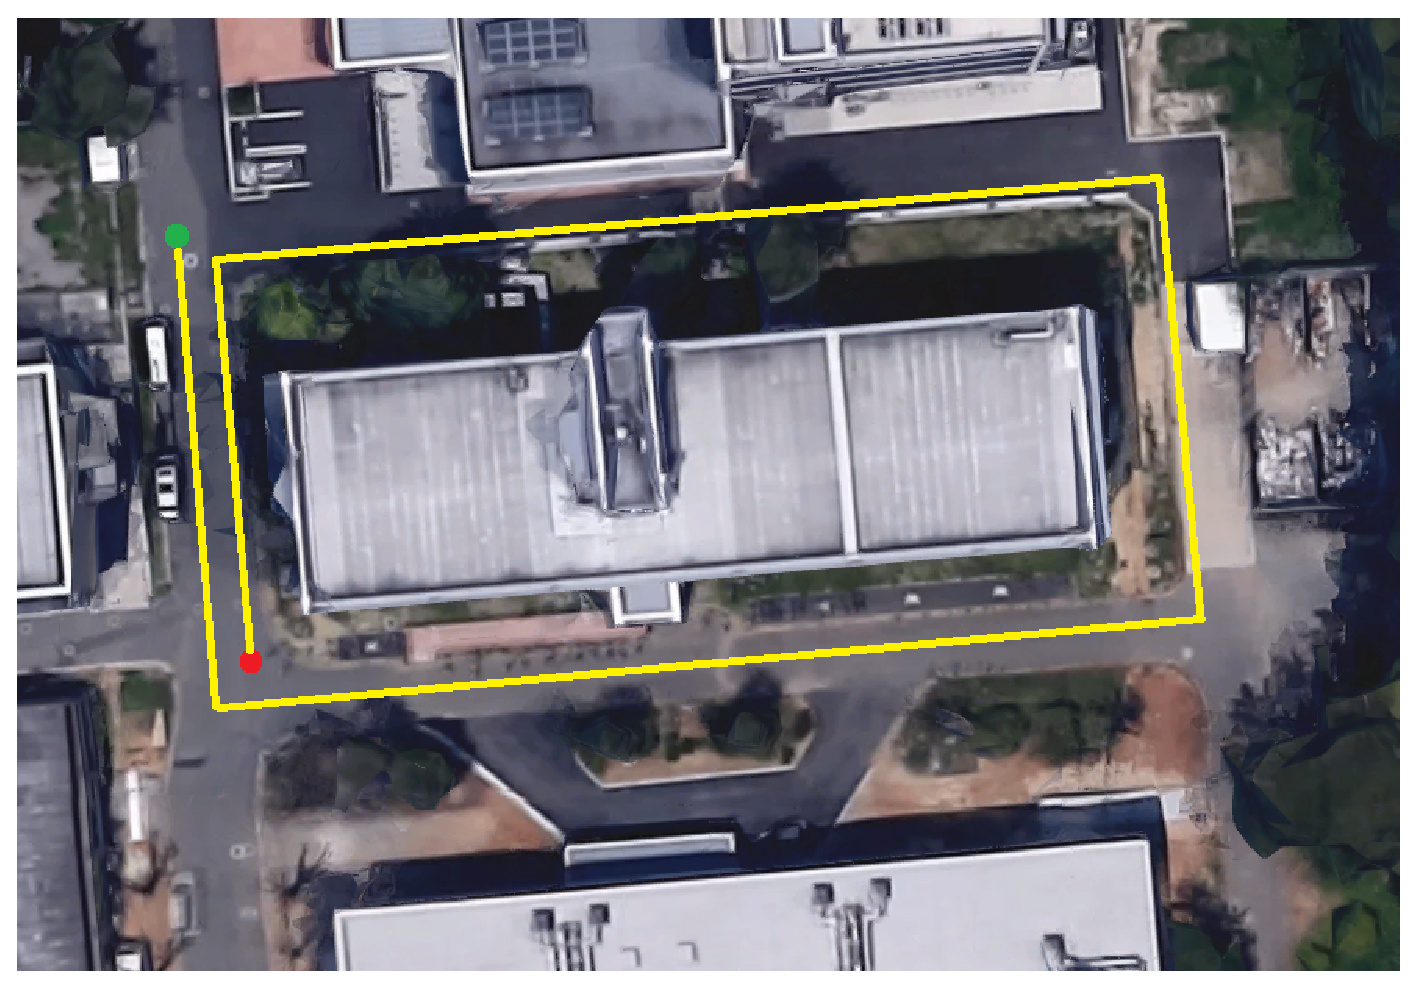
\includegraphics [width=9cm] {./fig/soukoukeiro2017.eps}
\end{tabular} 
\caption{$BAv9T7PO)(B}\label{$BAv9T7PO)(B}
\end{figure}

\begin{comment}
\newpage
GPS$B%G!<%?$OKL0^!$El7P!$1R@1JdB-?t$H$7$FF@$i$l$k!%(BGPS$B:BI8$r@$3&:BI8$X$HJQ49$9$k!%;~9o(B$k$$B$G$NKL0^!$El7P$r(B$\acute{N}_{k}$$B!$(B$\acute{E}_{k}$$B$H$9$k$H!$El7P$NJQ49$O(B
\begin{equation}
 \acute{x}_{k}
  =(\acute{E}_{k}-\acute{E}_{0})
  \frac{\beta}{360}\
  \cos\left(\frac{\pi\acute{N}_{0}}{180}\right)
\end{equation}
$B$H$J$k!%$3$3$G(B$\beta$$B$O@VF;D9$G(B$40075.017$[km]$B$G$"$k!%F1;~$KKL0^$O(B
\begin{equation}
 \acute{y}_{k}=(\acute{N}_{k}-\acute{N}_{0})\frac{\pi\gamma}{360}
\end{equation}
$B$H$J$k!%$3$3$G(B$\gamma$$B$OKL6K$HFn6K$r7k$s$@D>7B$G(B$12756.274$[km]$B$G$"$k!%(B
\par
\end{comment}

\newpage
 \subsection{$B<B837k2L$H9M;!(B}
$B!!(B\subsubsection{PF$B$K$h$k?dDj7k2L$H9M;!(B}
   \begin{comment}
$B<B837k2L$r$&$1$F!$(BGPS$B$N8m:9860x$K$D$$$FD4$Y$k$?$aDI<B83$r9T$C$?!%@h9T8&(B
$B5f$G$O(B3$B9fEo<~JU$G$N%G!<%?<hF@$N:]$K!$K\<B83$GF@$i$l$?$h$&$J(B
$B%i%s%@%`%N%$%:$N1F6A$7$?$h$&$J%G!<%?$OF@$i$l$F$$$J$+$C$?!%$=$3$G!$(BKinect
$B$rEk:\!$;HMQ$9$k$3$H$K$h$C$F%N%$%:$,@8$8$?2DG=@-$r9M$(8!>Z$r9T$C$?!%(B
$B?^(B\ref{Kinect$B$rEk:\$7$J$$>l9g(B}$B!$?^(B\ref{Kinect$B$rEk:\$7;HMQ$7$J$$>l9g(B}
$B$O$=$l$>$l(BKinect$B$rEk:\$7$J$$>l9g$H(BKinect$B$rEk:\$7;HMQ$7$J$$>l(B
$B9g$N!$(BGPS$B%G!<%?<hF@7k2L$G$"$k!%7PO)$OK\<B83$r9T$C$?7PO)$HF1$87PO)$rK\<B(B
$B83$HO"B3$7$FAv9T$5$;$?!%(B\par
$B7k2L(BKinect$B$r;HMQ$7$J$+$C$?(B2$B$D$NDI<B83$G$O!$%i%s%@%`%N%$%:$N1F6A$7$?$h$&(B
$B$J7PO)$O$_$i$l$J$+$C$?!%$h$C$F!$(BKinect$B$r;HMQ$9$k$3$H$K$h$k?.9f$dEEGH$N(B
$B43>D$,860x$G$"$k$H?dB,$9$k!%(B

\begin{figure}[p]
 \begin{center}
  \begin{tabular}{cc}
   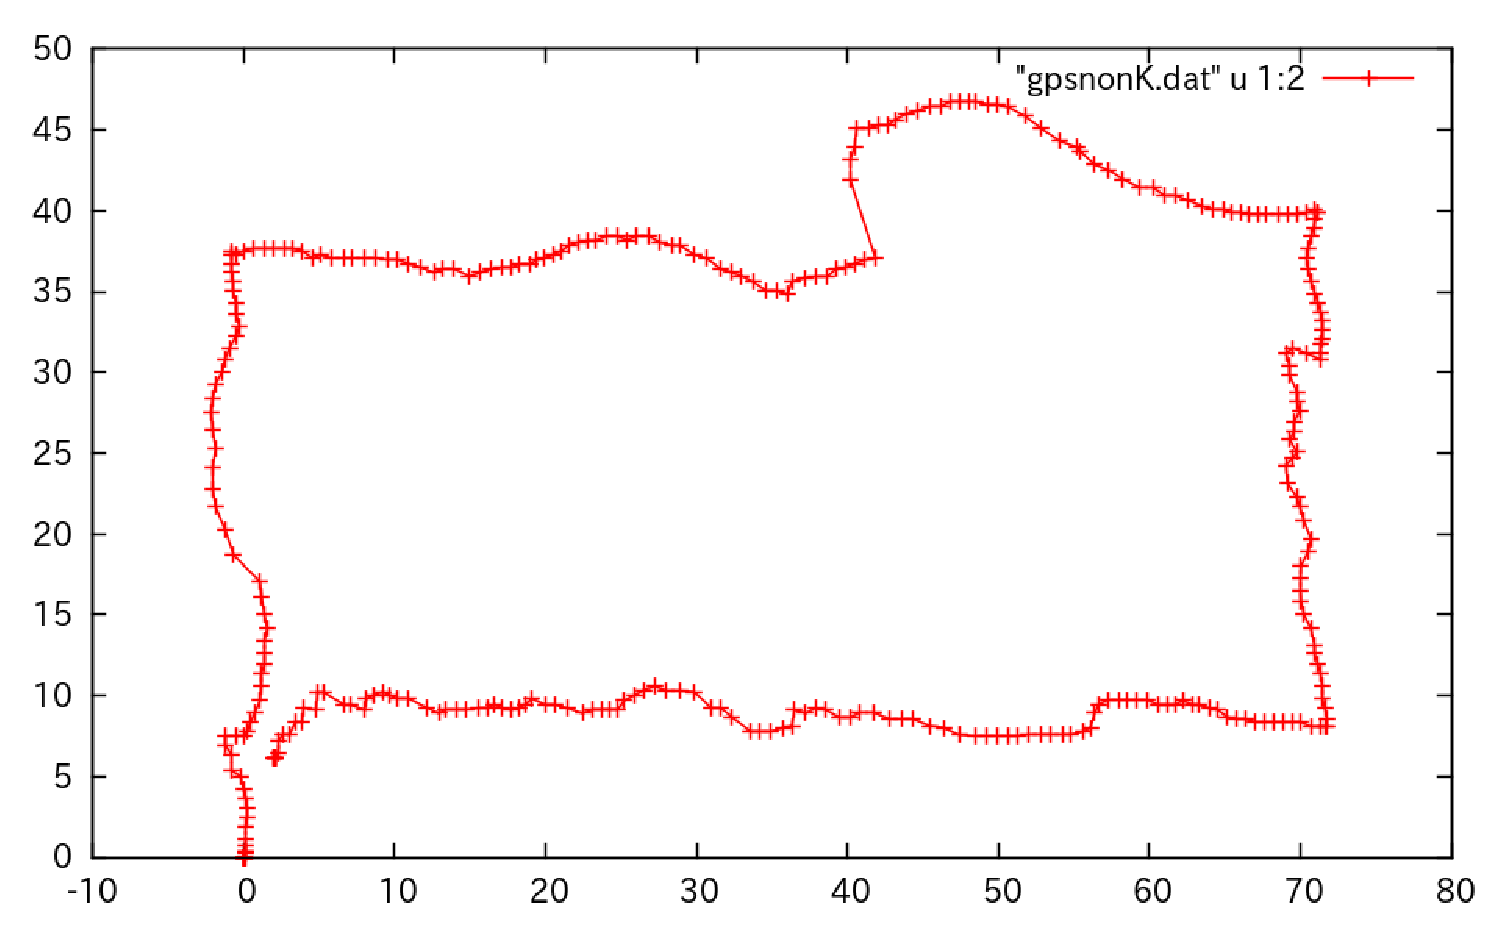
\includegraphics [width=10.0cm] {./fig/gps1.eps}
   \end{tabular}
  \end{center}
 \caption{Kinect$B$rEk:\$7$J$$>l9g(B}\label{Kinect$B$rEk:\$7$J$$>l9g(B}
\end{figure}

\begin{figure}[p]
 \begin{center}
  \begin{tabular}{cc}
   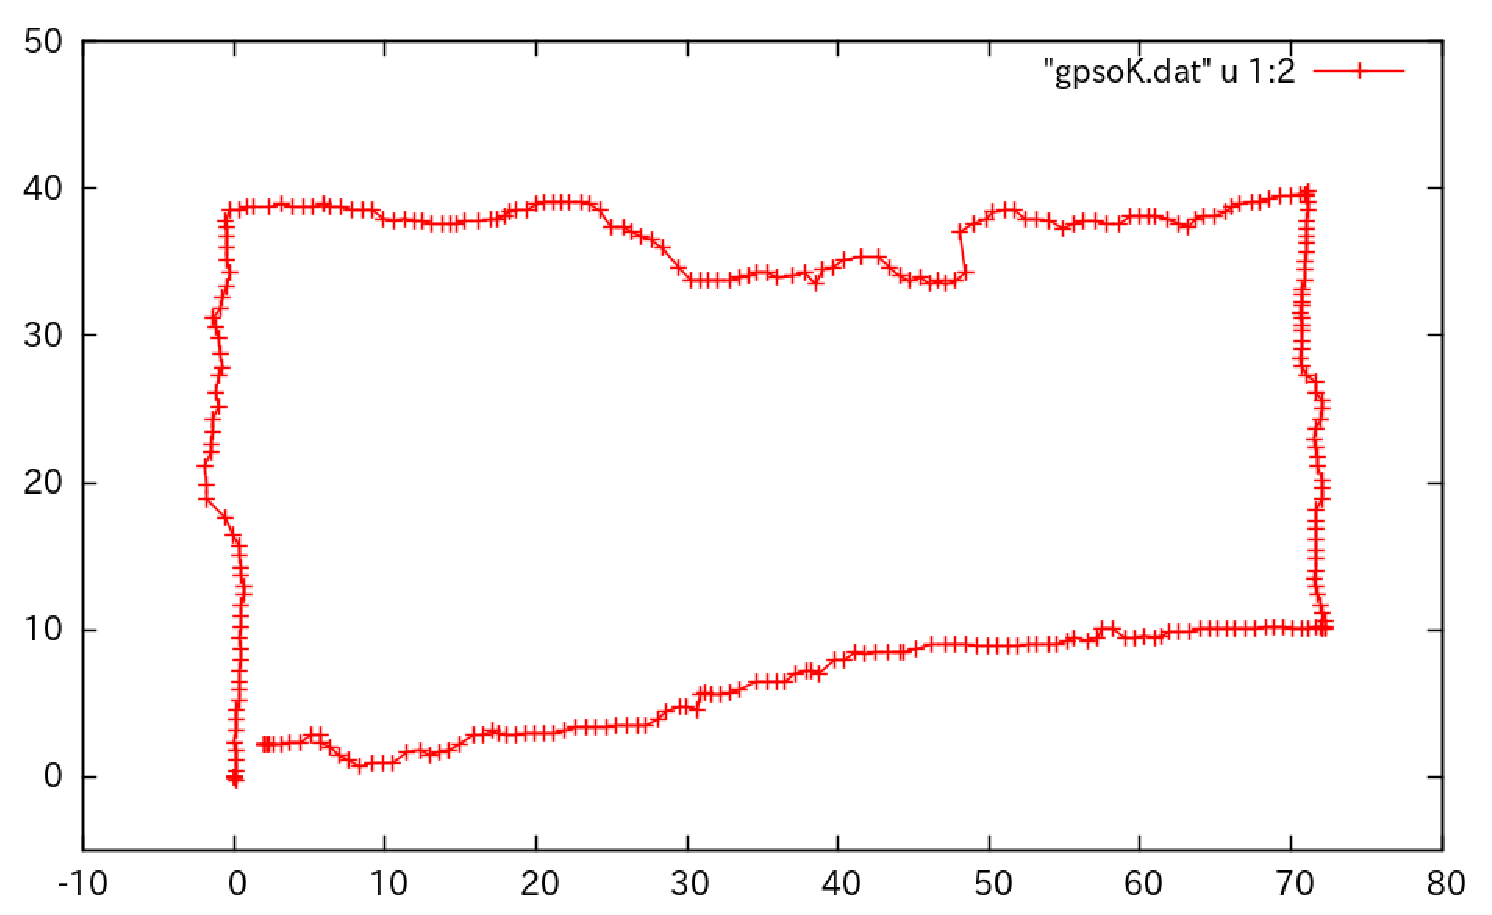
\includegraphics [width=10.0cm] {./fig/gps2.eps}
   \end{tabular}
  \end{center}
 \caption{Kinect$B$rEk:\$7;HMQ$7$J$$>l9g(B}\label{Kinect$B$rEk:\$7;HMQ$7$J$$>l9g(B}
\end{figure}
\end{comment}

\newpage


\section{$B7kO@(B}\typeout{=== Region from (point) to (mark) ===}

\end{document}
